\section{Which Material Cues Survive Conversion?}
\label{app:materials}

The three-condition comparison places original MDL, ConvertAsset, and the
NVIDIA PreviewSurface conversion route side by side. The selected GRScenes
cases cover opacity or transparency, emission, normal or bump mapping, and
displacement or height. Figure~\ref{fig:app-materials} shows matched renders;
Table~\ref{tab:app-materials} reports the corresponding static inventory.
A sample may contain several effects, so the effect counts overlap.

\begin{table}[htbp]
\centering\small
% Generated by appendix/build_tables.py; source hashes in table_sources.json.
\begin{tabular}{lrrrr}
\toprule
Effect & $N$ & Original & ConvertAsset & NVIDIA \\
\midrule
Clearcoat fixture & 1 & 1/1 & 1/1 & 0/1 \\
Opacity / transparency & 7 & 7/7 & 7/7 & 7/7 \\
Emission & 26 & 26/26 & 26/26 & 26/26 \\
Procedural fixture & 1 & 1/1 & 1/1 & 1/1 \\
Normal / bump & 30 & 30/30 & 30/30 & 30/30 \\
Displacement / height & 26 & 26/26 & 26/26 & 26/26 \\
\bottomrule
\end{tabular}

\caption{Material-effect inventory. Entries count outputs passing the recorded
static checks over selected samples. Converted outputs are checked for target
presence and zero active MDL; visual appearance is examined in the paired
panels. The two fixtures are listed separately from the GRScenes samples.}
\label{tab:app-materials}
\end{table}

The four GRScenes effect groups produce statically usable outputs for both
conversion routes. Their renders make the remaining appearance differences
visible: loading a material successfully is only one part of preserving the
cues a model receives. The shared columns let readers compare the target and
its context directly, without interpreting the effect inventory as a
perceptual score.

\subsection{Clearcoat and procedural texture}
The two fixtures in Figure~\ref{fig:app-material-failures} isolate concrete
failure modes. In the clearcoat fixture, the NVIDIA-converted stage lacks the
target prim. ConvertAsset retains the target but approximates its material;
the recorded review flags the changed blue/clearcoat appearance. In the
procedural-texture fixture, both converted stages retain the target, yet the
authored checker pattern is lost. This second case is particularly instructive:
static target and shader checks pass while a salient surface pattern disappears.

These fixtures explain why the grounding study uses rendered comparisons in
addition to checking scene structure. They identify specific losses in the
tested outputs; the selected examples do not estimate how often those losses
occur across a material library.

\begin{figure}[htbp]
\centering
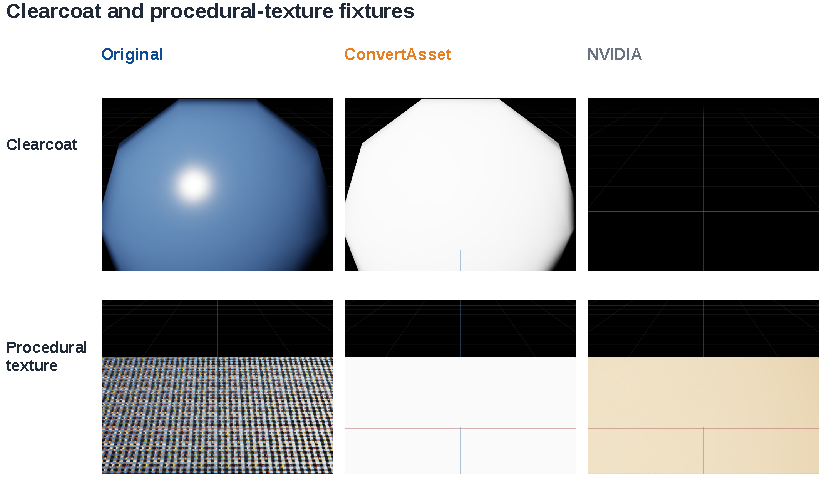
\includegraphics[width=\linewidth,height=.84\textheight,keepaspectratio]{appendix_material_failures.pdf}
\caption{Clearcoat and procedural-texture fixtures under the three material conditions. The NVIDIA clearcoat output loses the target; both converted procedural outputs lose the checker pattern. ConvertAsset retains the clearcoat target with an altered appearance.}
\label{fig:app-material-failures}
\end{figure}
\begin{figure}[p]
\centering
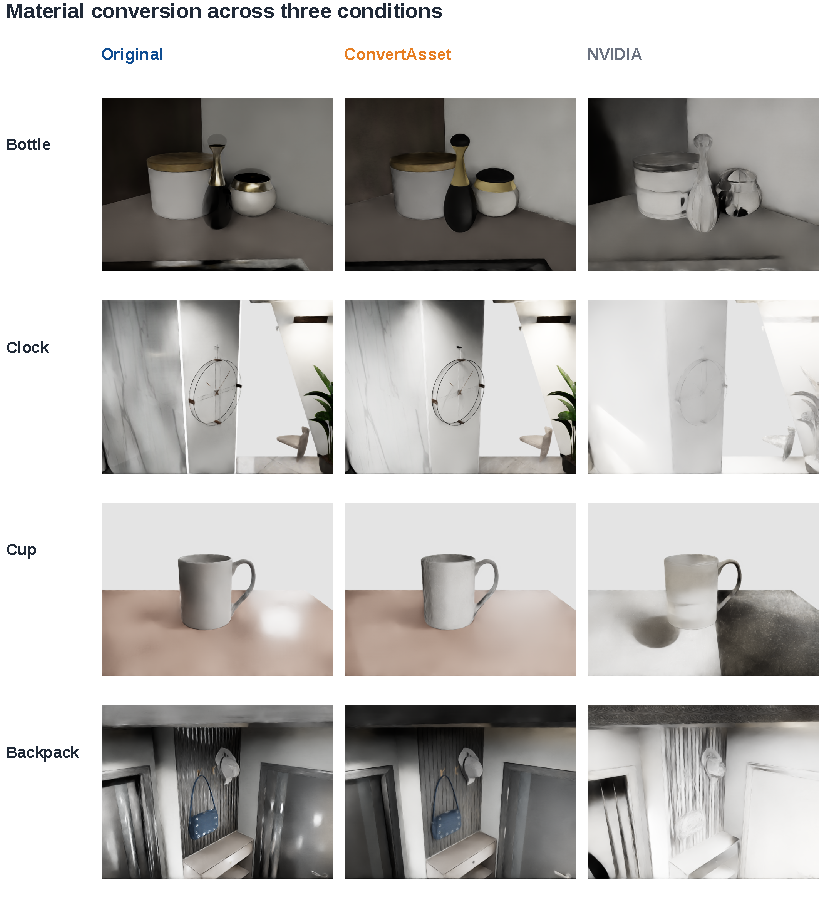
\includegraphics[width=\linewidth,height=.84\textheight,keepaspectratio]{appendix_material_comparison.pdf}
\caption{Matched material examples across original MDL, ConvertAsset, and NVIDIA conversion. Rows show a bottle, clock, cup, and backpack. These selected examples contain overlapping material effects; Table~\ref{tab:app-materials} reports the effect inventory.}
\label{fig:app-materials}
\end{figure}

\FloatBarrier
